\documentclass{article}
\usepackage{latexsym}
\usepackage{amsmath}
\usepackage{amssymb}
\usepackage{amsthm}
\usepackage{graphicx}

\newtheorem{theorem}{Theorem}[section]
\begin{document}
\title{"Fermat's" Two Squares (aka Christmas) Theorem}
\author{Dave Neary}

\maketitle

\section{Fermat's Two Primes Theorem}

The theorem states that an odd prime $p$ can be written as the sum of two squares of
positive integers:
\[ p = a^2 + b^2 , a, b \in \mathbb{N} \]
if and only if it is of the form $4k+1, k\in \mathbb{N}$.

This theorem was stated by Fermat without proof, and it was several decades before a proof
was provided. Since then, several proofs have been discovered, including one which relies 
on the characteristics of the Gaussian integers, and another which we can prove using a
very pretty geometry-based involution. I present these two proofs (with dependent tools)
below.

\section{Dedekind's Proof in Gaussian Integers}

\subsection{Gaussian Integers}

The Gaussian integers $\mathbb{Z}[i]$ are complex numbers of the form 
\[ \mathbb{Z}[i] = \{a+ib:a,b\in \mathbb{Z}, i=\sqrt{-1}\}\]

The Gaussian integers are closed under the standard multiplication operator
$(a+ib) \times (c+id) = (ac-bd) + i(bc+ad)$, which is commutative (meaning
$z_1 \times z_2 = z_2 \times z_1$), and they have a multiplicative and additive
identity. They are therefore a ring.

By defining a norm function $N(a+bi) = a^2+b^2$, we can also define Euclidean division of
Gaussian integers. That is, for $a,b \in \mathbb{Z}[i]$, there exist $q,r \in \mathbb{Z}[i],
\text{ s.t. } a=qb+r, \text{ with } N(r)<N(b)$. So we can use classic division
algorithms like  the Euclidean algorithm and Bézout's itentity on Gaussian integers. This
characteristic means that $\mathbb{Z}[i]$ is a Euclidean domain, and, as a result, a Unique
Factorization Domain.

What this means is that, given any element $x \in \mathbb{Z}[i]$, we can find a unique
factorization of $x$ in irreducible elements $\{p_i\}$ and a unit $u$ such that:
\[ x = up_1p_2\cdots p_n \text{ with } n\geq 0 \]

In the ring of integers, we call these irreducible elements primes, and in the Gaussian
integers, we will call them Gaussian primes. The Gaussian integers has four units,
$\pm 1, \pm i$.

\subsection{Fermat's Little Theorem}

For the Two Squares theorem, we will be using a sub-ring of the Gaussian integers, the
Gaussian integers $\pmod{p}$ defined as $\{a+ib:a,b\in \mathbb{Z}/p\mathbb{Z}, i=\sqrt{-1}\}$.
Again, this set is closed under multiplication and addition, and we will denote the set 
$\mathbb{Z}[i]/(p)$. The notation $(p)$ denotes a prime ideal of the Gaussian integers - the
subset of the Gaussian integers that can be generated from the irreducible element $p$.

We will need some well-known results from modular arithmetic to complete the proof. The first
of these is Fermat's Little Theorem, which states:

\begin{theorem}For every prime $p \in \mathbb{N}$, and $a \in \mathbb{N}$ :
\[ a^p \equiv p \pmod{p} \]
\end{theorem}

\begin{proof}
If $a\equiv 0 \pmod{p}$ then $a^p \equiv 0 = a \pmod{p}$

If $\gcd(a,p)=1$: 
\[a \times n \equiv a \times m \pmod{p} \implies a(n-m) \equiv 0 \pmod{p} \]

Since $\gcd(a,p)=1$: $n-m\equiv 0 \pmod{p} \implies n = m \pmod{p}$. Therefore:

\[ \{i: 0 < i < p, i \in \mathbb{N}\} = \{a\times i, 0 < i < p, i \in \mathbb{N} \} \]

That is, the set of the non-zero integers mod $p$ is a derangement of itself when we 
multiply each element by any member of the set, so if we multiply all of the elements
together we get the same number. That is:

\[ \prod_{i=1}^{p-1} i \equiv \prod_{i=1}^{p-1} a\times i \]
\[ (p-1)! \equiv a^{p-1}\times (p-1)! \]

And since all numbers in $(p-1)!$ are relatively prime to $p$, we can divide across on both sides to
leave: $1 \equiv a^{p-1}$
\end{proof}

We will use this result to identify a criterion for identifying numbers that can square to a 
certain value.

\subsection{Quadratic residues and the Euler criterion}

Fermat's Little Theorem proves that all numbers $\pmod{p}$ have a multiplicative order of at
most $p-1$, but clearly there are numbers with a smaller order. For example, $1^i = 1$ for all
$i$, and $(-1)^i = 1$ for all even $i$.

Quadratic residues in $\mathbb{Z}/p\mathbb{Z}$ are numbers which have a square root in
$\mathbb{Z}/p\mathbb{Z}$. For example, in $\mathbb{Z}/5\mathbb{Z}$, $1^2 \equiv 4^2 \equiv 1
\pmod{5}$, and $2^2 \equiv 3^2 \equiv 4 \pmod{5}$, so $\{1,4\}$ is the set of quadratic residues
$\pmod{5}$. We can show that for a prime $p$, exactly $\frac{p+1}{2}$ of the members of
$\mathbb{Z}/p\mathbb{Z}$ are quadratic residues (including 0), and $\frac{p-1}{2}$ are quadratic
non-residues.

In particular, 1 has two square roots $\pmod{p}: \pm 1$. If we can show that 
\[\sqrt{a^{p-1}} = a^{\frac{p-1}{2}} = 1\]
then that implies that there is some number $m \in \mathbb{Z}/p\mathbb{Z}$ such that $m^2 = a$,
since $m^{p-1} = 1$ for all $m \neq 0$. This test for quadratic residues is called Euler's
criterion, and is formally defined for odd primes as:
\[a^{\frac{p-1}{2}} =
\left\{
	\begin{array}{ll}
		1  & \mbox{if there exists } m \in \mathbb{Z}/p\mathbb{Z} \mbox{ such that } m^2 \equiv a \pmod{p} \\
		-1  & \mbox{if } a \mbox{ is a quadratic non-residue in } \mathbb{Z}/p\mathbb{Z} \\
	\end{array}
\right. \]

\subsection{The Two Primes Theorem}

We now have all of the tools we need to prove the Two Primes theorem.

First, it is trivial to prove that no prime of the form $4k+3$ can be written as the sum of two
squares by noticing that $n^2 \equiv 0 \mbox{ or } 1 \pmod{4}$ for all $n\in \mathbb{N}$, so 
$a^2+b^2 = 0,1 \mbox{ or } 2 \pmod{4}$, but $p \equiv 3 \pmod{4}$.

Now, for $p=4k+1$, we must show that there exist $a,b \in \mathbb{N}$ such that $p=a^2+b^2$. There
is a second question, regarding the uniqueness of this solution, which we will not prove here.

Note that $(-1)^{\frac{p-1}{2}} = 1$ since $\frac{p-1}{2}=2k$, so -1 is a quadratic
residue $\pmod{p}$. Therefore, there must be an $a \in \mathbb{Z}/p\mathbb{Z}$ such that
$a^2 + 1 \equiv 0 \pmod{p}$. Now, in $\mathbb{Z}[i]/(p)$, we can factor $a^2+1$ into
$(a-i)(a+i)$. Since $N(a+i)=N(a-i)<N(p)$ (since $a < p$), $p$ does not divide either $a+i$ or
$a-i$, and therefore, $p$ is not a prime in $\mathbb{Z}[i]/(p)$, so there exists some Gaussian 
prime factorization of $p = (x+iy)(x-iy)$ - giving $p = x^2+y^2$.

I like this proof, because once we know that the Gaussian integers are a UFD, we can use all of
the other tools we get from modular arithmetic to show that $p$ must have non-trivial factors.
However, understanding the proof does require an understanding of modular arithmetic and rings.

\section{Zagier's one sentence proof}

The following proof uses a transformation which appears to come from out of nowhere, but as we
shall see, has a very intuitive geometric explanation. The full statement of the proof is:

Let $p=4k+1$ be prime, let $\mathbb{N}$ denote the natural numbers, and consider the finite set
$S=\{(x,y,z) \in \mathbb{N}^3: x^2+4yz = p\}$ of triples of numbers. Then $S$ has two 
involutions: $(x,y,z) \to (x,z,y)$ with fixed points when $y=z$ (corresponding to 
$p=x^2+(2y)^2$ a sum of two squares) and the following:
\[ (x,y,z) \to
\left\{
	\begin{array}{ll}
		(x+2z,z,y-x-z)  & \mbox{if } x< y-z \\
		(2y-x,y,x-y+z)  & \mbox{if } y-z < x < 2y \\
		(x-2y,x-y+z,y)  & \mbox{if } x > 2y \\
	\end{array}
\right. \]
which has exactly one fixed point at $(x,y,z) = (1,1,k)$. Two involutions over the same
set must have sets of fixed points of the same parity, and since the second involution
has exactly one fixed point, the first involution must have at least one fixed point, so
$p$ must be expressible as the sum of two squares.

\subsection{Involutions}

The key to this proof is understanding involutions, and their fixed points. An involution
is simply a function which is its own inverse, that is, $x = f(f(x))$. Every involution is
a bijection - that is, every element of the range has an element of the domain that maps
onto it, and every element of the domain maps onto a different element of the range.

As a result, points in a set can have an order of 1 ($f(x)=x$, or $x$ is a fixed point
of $f$) or 2 ($f(x)=y, y(y)=x, x\neq y$) under an involution.

If you have two involutions on the same set, then if there is one fixed point in the first,
that means that the total number of solutions is odd (one fixed points and $k$ pairs of
points of order 2).

Then if there is a second involution, that must also apply to the same odd number of
elements of the set, and as a result, there must be an odd number of fixed points in this second involution too (specifically, at least one fixed point)

But where did that very complicated mapping come from? The time has come to talk about
windmills.

\subsection{Geometric representation of triples $(x,y,z)$}

Let's tease apart the "one-line" proof to see what's going on graphically.

First, let us verify that the involutions actually make sense.

For the members of the set $S=\{(x,y,z):p=x^2+4yz, x, y, z \in \mathbb{N}\}$, since
$p = 4k+1$, and $4yz$ is even, $x$ can be any odd number less than
$\sqrt{p}$. Since we are guaranteed that $x=2a+1$ for $a\in \mathbb{N}_0$, we can be
sure that $p-x^2 = 4k+1 -(4a^2+4a+1) = 4(k-a^2-a)$ is a multiple of 4, with $k>a^2+a$.
$(x,y,z) \in S \implies (x,z,y) \in S$ - so we are guaranteed that the first
transformation is an involution.

For the second transformation, we can consider a triple $(x,y,z)$ as a geometric
arrangement of a square of side $x$, plus four equal rectangles of size $y\times z$
arranged symmetrically around the central square. In the diagram below \ref{fig:windmill1},
we have one mapping for $p=89$ with $(x,y,z)=(5,8,2)$ mapping to $(x,y,z)=(9,2,1)$ under the
mapping $(x,y,z) \to (x+2z,z,y-x-z)$, and the inverse transformation corresponding
to $(x,y,z) \to (x-2y,x-y+z,y)$. The shapes we see for this form are the windmill
forms the proof is known for.

\begin{figure}
	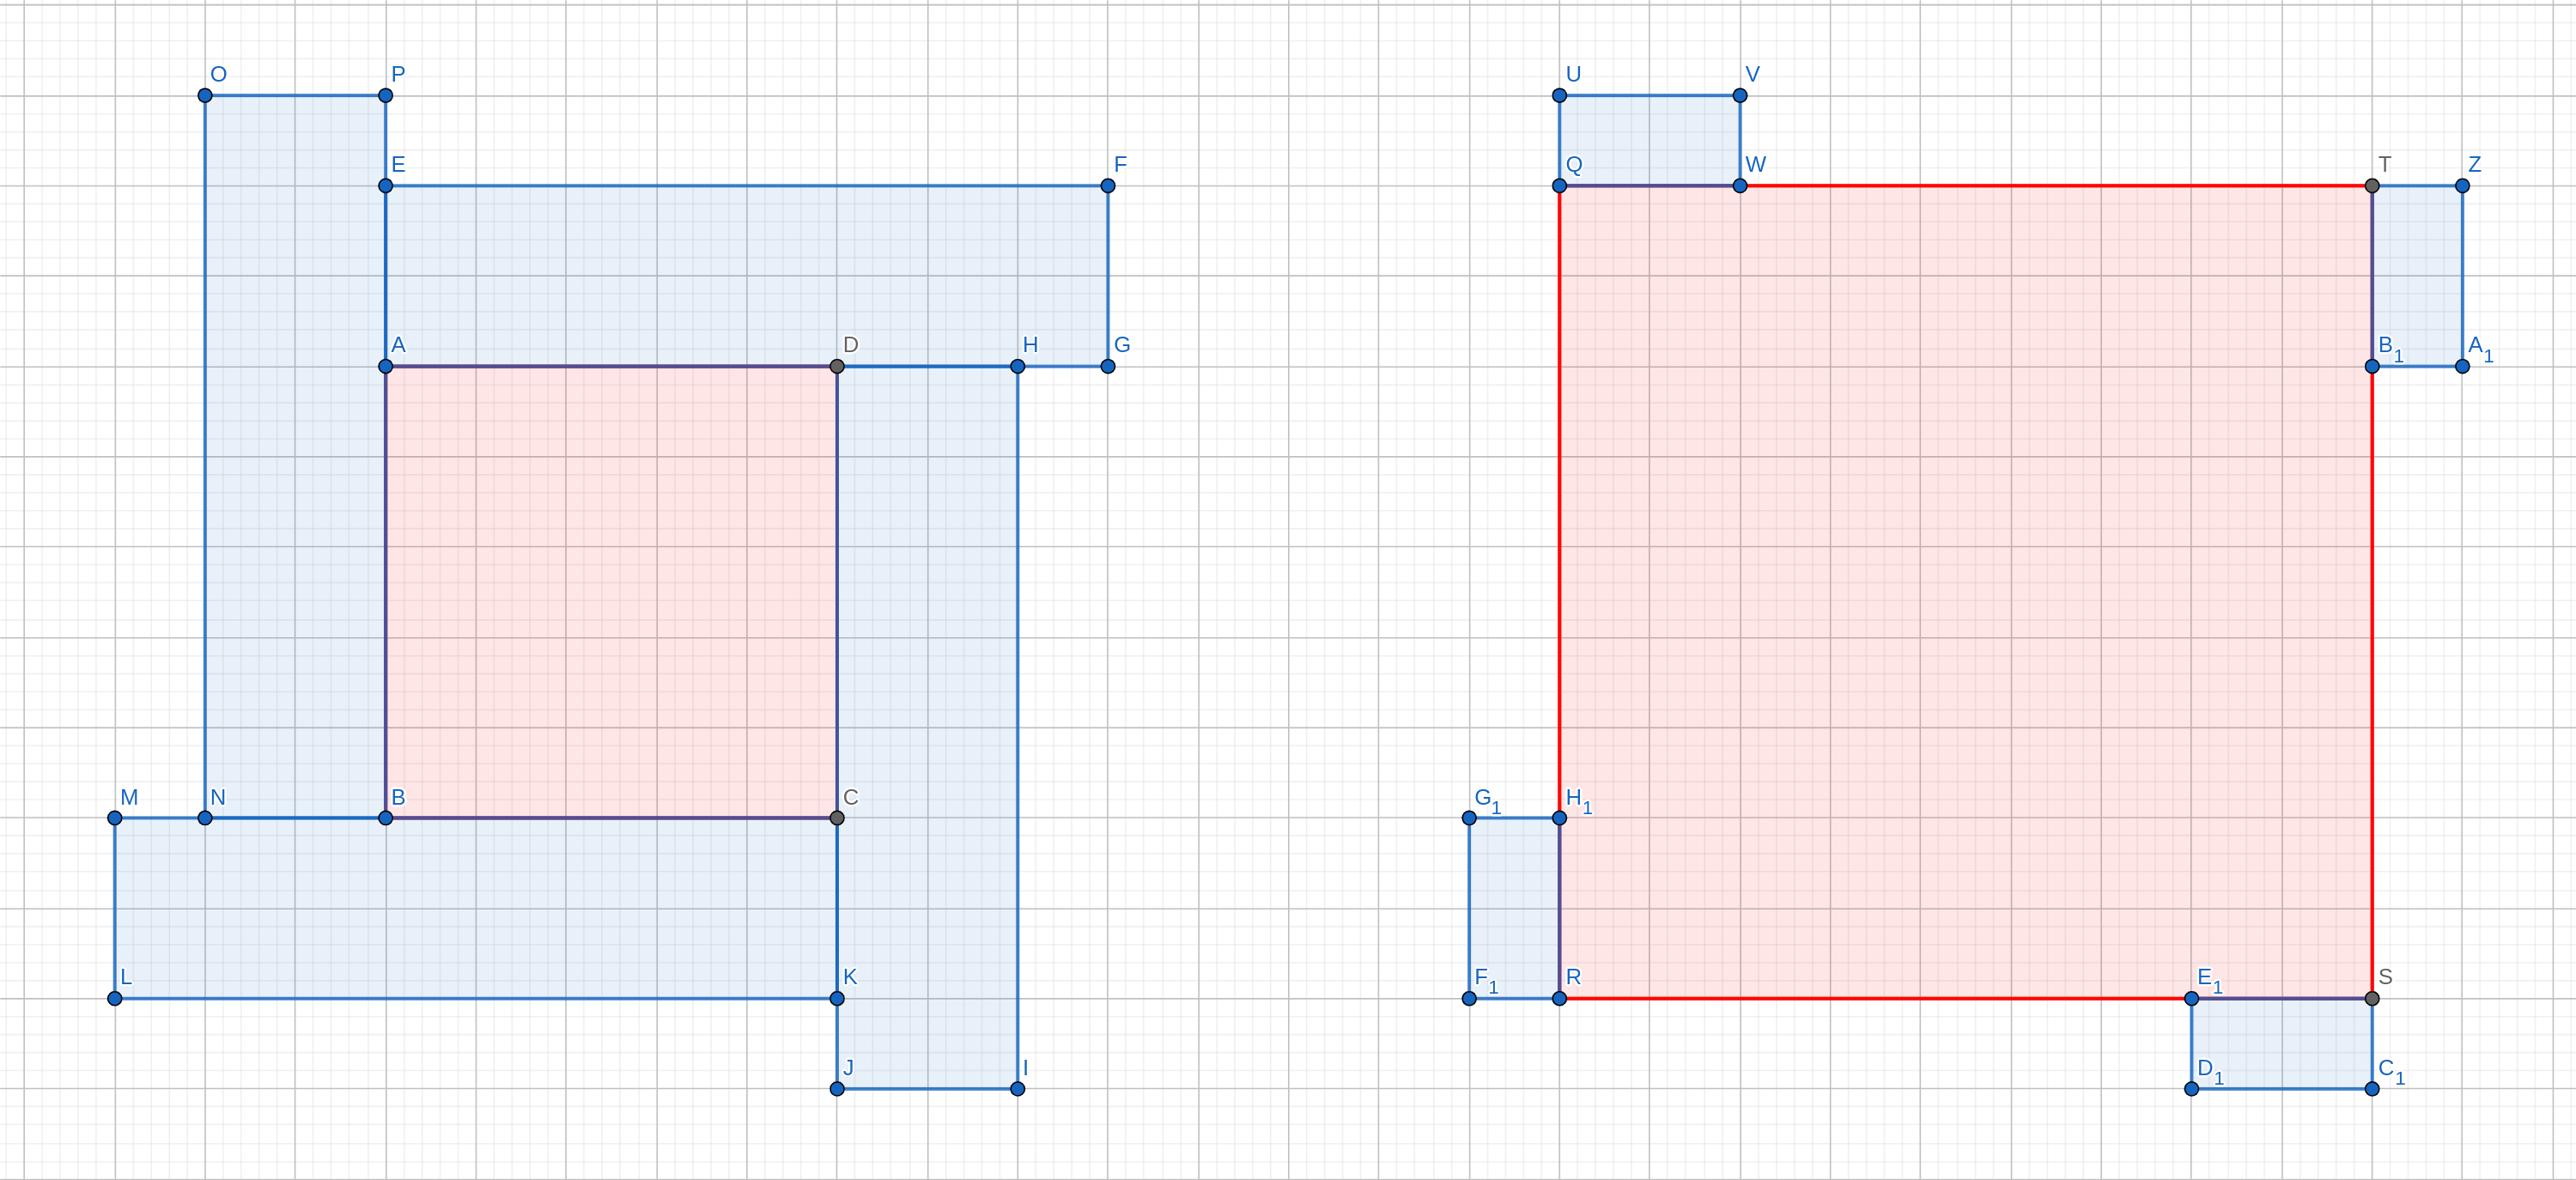
\includegraphics[width=\linewidth, bb=0px 0px 800px 400px]{windmill1.png}
	\caption{Mapping $(5,8,2) \to (9,2,1)$}
	\label{fig:windmill1}
\end{figure}

To show an alternative arrangement, we can swap $y$ and $z$ in the initial arrangement
to get $(x,y,z)=(5,2,8)$, which transforms under the rule $(x,y,z) \to (x-2y, x-y+z, y)$
to $(x,y,z) = (1, 11, 2)$, and transforms under the inverse rule $(x,y,z) \to 
(x+2z, z, y-x-z)$ (and note that at each stage, $x^2+4yz = 89$). In this arrangement,
the windmill pattern is clearer.


\begin{figure}
%	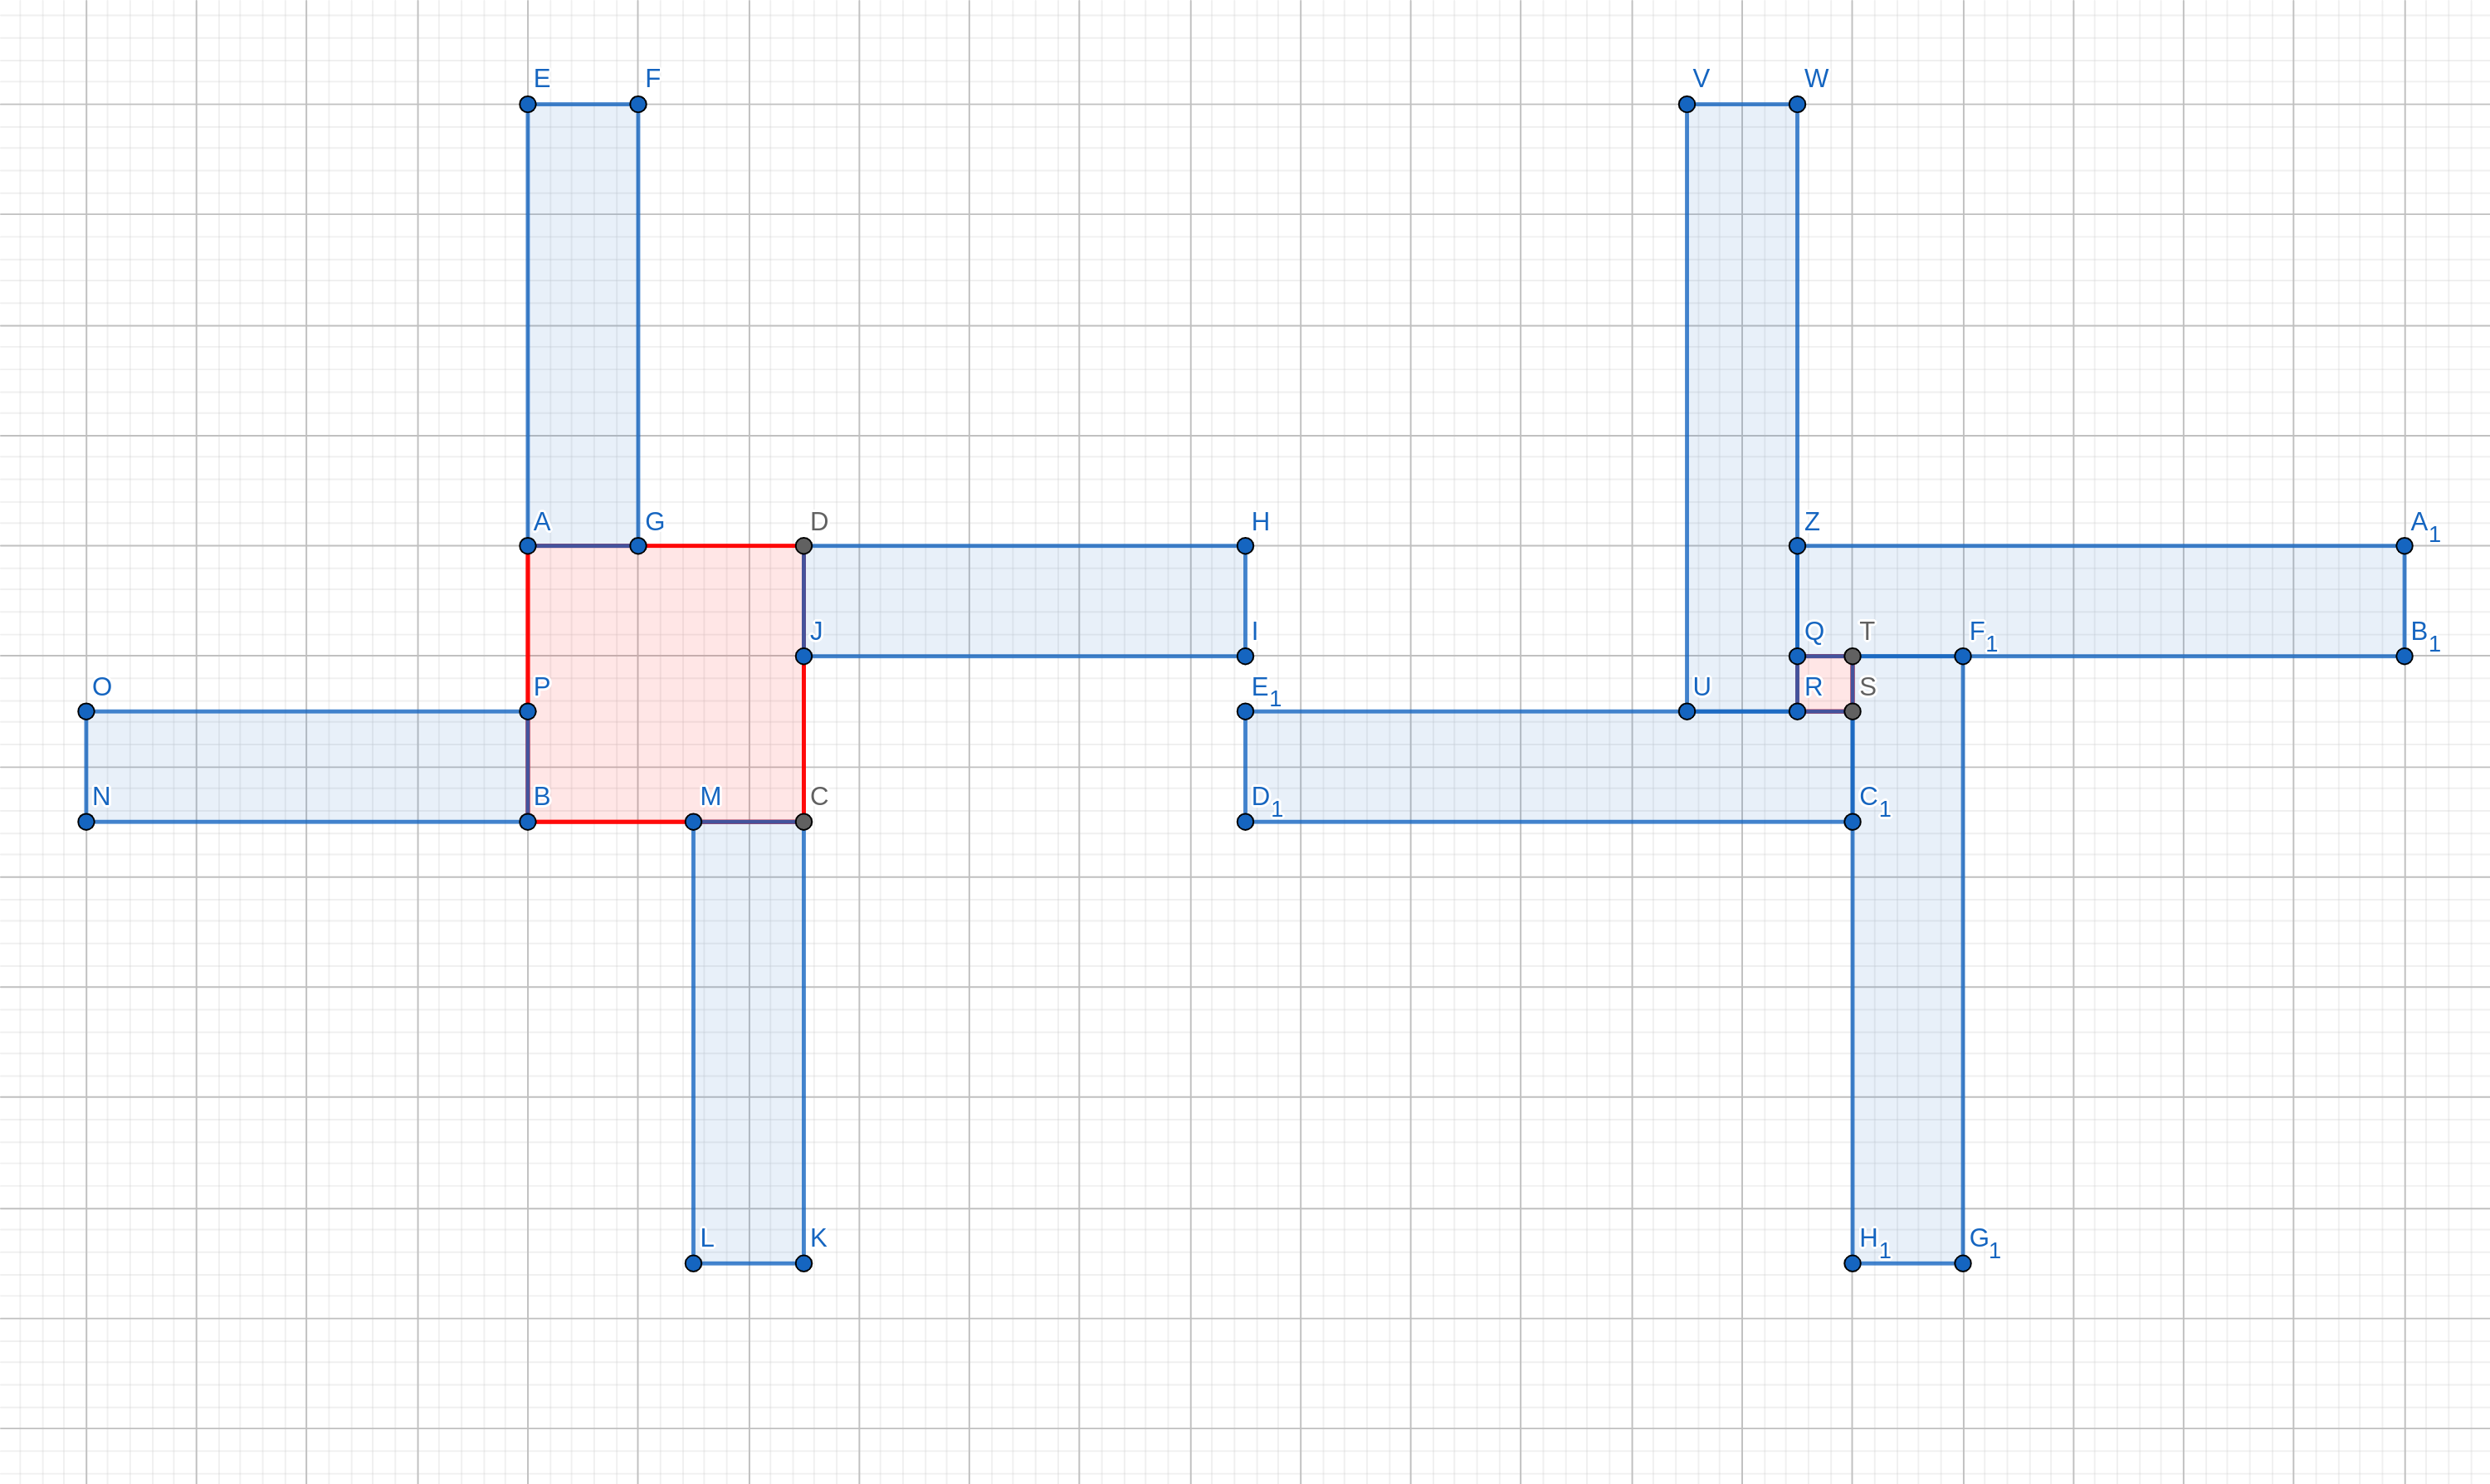
\includegraphics[width=\linewidth, bb=0px 0px 1200px 715px]{windmill2.png}
	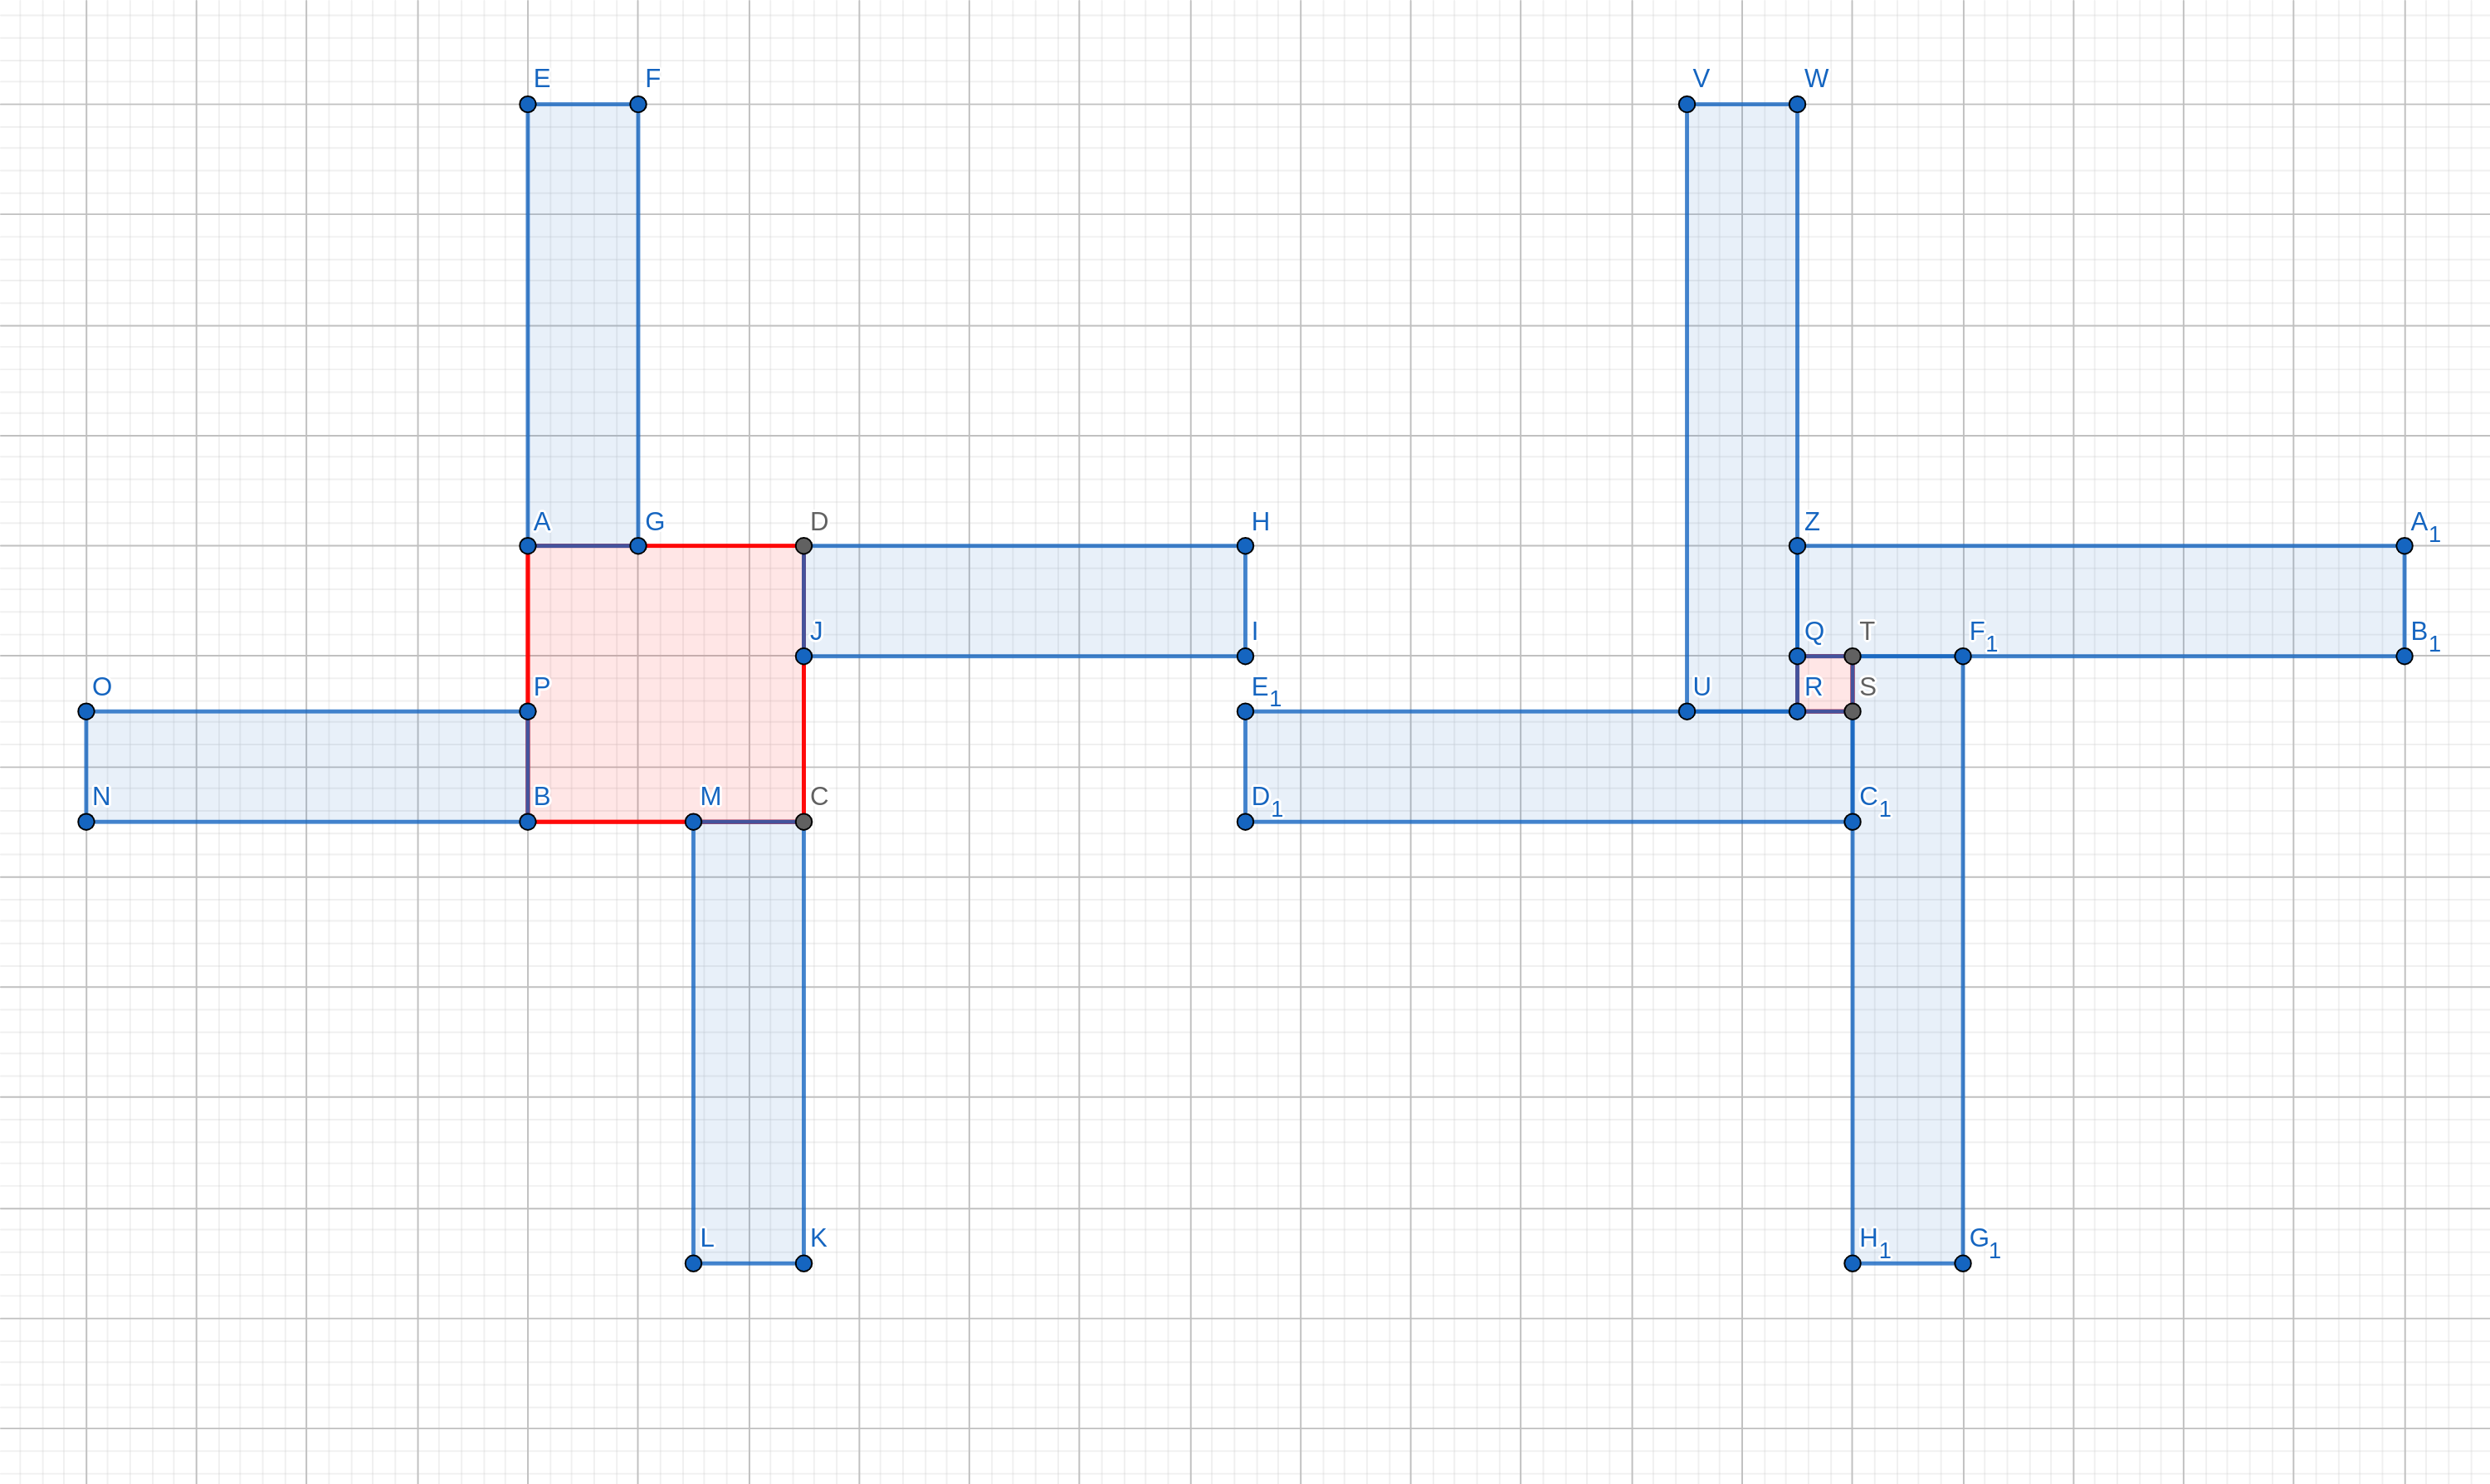
\includegraphics[width=\linewidth, viewport=0px 0px 1200px 715px]{windmill2.png}
	\caption{Mapping $(5,2,8) \to (1,11,2)$}
	\label{fig:windmill2}
\end{figure}

There are exactly two representations in $(x,y,z)$ for each shape
which is a solution to $p=x^2+4yz$, representing different ways of "wrapping" the
rectangles around the inside square, except for one representation, which is represented
by $(x,y,z) = (1,1,k)$ - this shape is a 1x1 square in the center, and four long and thin
rectangles pointing out at each side. For this configuration, there is no alternative way
to get a larger central square - this is guaranteed to be the only fixed point of the
transformation (since $y-z < x < 2y$, the rule $(x,y,z) \to (2y-x, y, x-y+z)$ is applied).

And going all the way back to our starting point, since we have exactly one fixed point
in this involution, and it is applied to the same set as the alternative involution,
the alternative must also have a fixed point. QED.


\appendix

\section{Using the Euclidean algorithm on $\mathbb{Z}[i]$}

We can find $\gcd(a,b), a,b \in \mathbb{Z}[i]$ using the Euclidean algorithm
as follows (example using $11 + 7i$ and $18 - i$):

\[N(11+7i) = 170, N(18-i)=324 \]

So we start with $18-i$ on the LHS.

\[ \frac{18 - i}{11 + 7i} = \frac{(18 - i)(11 - 7i)}{11^2+7^2} = \frac{205 - 137i}{170} \]

Rounding the real and imaginary parts to the nearest integers, we get 

\[ 18 - i = (1 - i)(11 + 7i) + 3i \]

Now we repeat with $11 + 7i, 3i$, noting that $N(3i) = 9$:

\[ \frac{11+7i}{3i} = \frac{(11 + 7i)(-3i)}{9} = \frac{7 -11i}{3} \]
\[ 11 + 7i = (2 - 4i)(3i) +i \]

And the GCD is the unit $i$ (or 1).

\end{document}

